%% Creator: Inkscape inkscape 0.48.5, www.inkscape.org
%% PDF/EPS/PS + LaTeX output extension by Johan Engelen, 2010
%% Accompanies image file 'RotSubparm.pdf' (pdf, eps, ps)
%%
%% To include the image in your LaTeX document, write
%%   \input{<filename>.pdf_tex}
%%  instead of
%%   \includegraphics{<filename>.pdf}
%% To scale the image, write
%%   \def\svgwidth{<desired width>}
%%   \input{<filename>.pdf_tex}
%%  instead of
%%   \includegraphics[width=<desired width>]{<filename>.pdf}
%%
%% Images with a different path to the parent latex file can
%% be accessed with the `import' package (which may need to be
%% installed) using
%%   \usepackage{import}
%% in the preamble, and then including the image with
%%   \import{<path to file>}{<filename>.pdf_tex}
%% Alternatively, one can specify
%%   \graphicspath{{<path to file>/}}
%% 
%% For more information, please see info/svg-inkscape on CTAN:
%%   http://tug.ctan.org/tex-archive/info/svg-inkscape
%%
\begingroup%
  \makeatletter%
  \providecommand\color[2][]{%
    \errmessage{(Inkscape) Color is used for the text in Inkscape, but the package 'color.sty' is not loaded}%
    \renewcommand\color[2][]{}%
  }%
  \providecommand\transparent[1]{%
    \errmessage{(Inkscape) Transparency is used (non-zero) for the text in Inkscape, but the package 'transparent.sty' is not loaded}%
    \renewcommand\transparent[1]{}%
  }%
  \providecommand\rotatebox[2]{#2}%
  \ifx\svgwidth\undefined%
    \setlength{\unitlength}{1200bp}%
    \ifx\svgscale\undefined%
      \relax%
    \else%
      \setlength{\unitlength}{\unitlength * \real{\svgscale}}%
    \fi%
  \else%
    \setlength{\unitlength}{\svgwidth}%
  \fi%
  \global\let\svgwidth\undefined%
  \global\let\svgscale\undefined%
  \makeatother%
  \begin{picture}(1,0.42)%
    \put(0,0){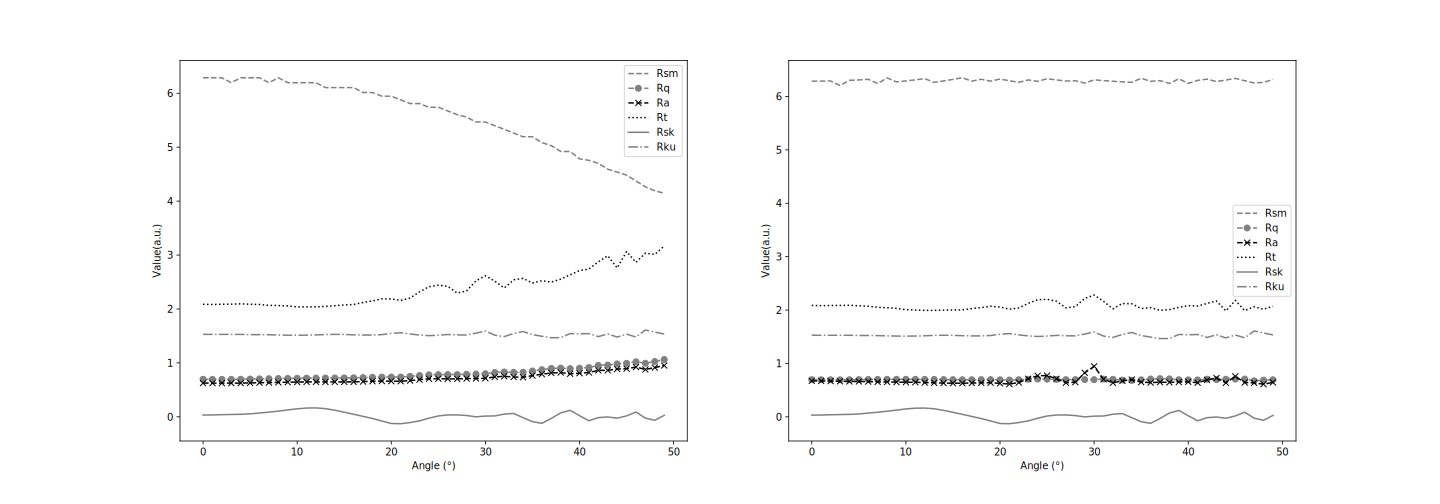
\includegraphics[width=\unitlength]{RotSubparm.pdf}}%
    \put(0.06307237,0.04033463){\makebox(0,0)[b]{\smash{0}}}%
    \put(0.14150045,0.04033463){\makebox(0,0)[b]{\smash{10}}}%
    \put(0.21992851,0.04033463){\makebox(0,0)[b]{\smash{20}}}%
    \put(0.29835658,0.04033463){\makebox(0,0)[b]{\smash{30}}}%
    \put(0.37678464,0.04033463){\makebox(0,0)[b]{\smash{40}}}%
    \put(0.45521268,0.04033463){\makebox(0,0)[b]{\smash{50}}}%
    \put(0.25522113,0.02893621){\makebox(0,0)[b]{\smash{Angle (°)}}}%
    \put(0.03802417,0.06948006){\makebox(0,0)[rb]{\smash{0}}}%
    \put(0.03802417,0.11442034){\makebox(0,0)[rb]{\smash{1}}}%
    \put(0.03802417,0.15936063){\makebox(0,0)[rb]{\smash{2}}}%
    \put(0.03802417,0.20430092){\makebox(0,0)[rb]{\smash{3}}}%
    \put(0.03802417,0.24924121){\makebox(0,0)[rb]{\smash{4}}}%
    \put(0.03802417,0.29418148){\makebox(0,0)[rb]{\smash{5}}}%
    \put(0.03802417,0.33912177){\makebox(0,0)[rb]{\smash{6}}}%
    \put(0.02765568,0.21105){\rotatebox{90}{\makebox(0,0)[b]{\smash{Value(a.u.)}}}}%
    \put(0.44083606,0.35576797){\makebox(0,0)[lb]{\smash{Rsm}}}%
    \put(0.44083606,0.3435362){\makebox(0,0)[lb]{\smash{Rq}}}%
    \put(0.44083606,0.33130444){\makebox(0,0)[lb]{\smash{Ra}}}%
    \put(0.44083606,0.31907265){\makebox(0,0)[lb]{\smash{Rt}}}%
    \put(0.44083606,0.30684088){\makebox(0,0)[lb]{\smash{Rsk}}}%
    \put(0.44083606,0.29460911){\makebox(0,0)[lb]{\smash{Rku}}}%
    \put(0.57034508,0.04033463){\makebox(0,0)[b]{\smash{0}}}%
    \put(0.64877317,0.04033463){\makebox(0,0)[b]{\smash{10}}}%
    \put(0.72720126,0.04033463){\makebox(0,0)[b]{\smash{20}}}%
    \put(0.80562935,0.04033463){\makebox(0,0)[b]{\smash{30}}}%
    \put(0.88405739,0.04033463){\makebox(0,0)[b]{\smash{40}}}%
    \put(0.96248543,0.04033463){\makebox(0,0)[b]{\smash{50}}}%
    \put(0.76249387,0.02893621){\makebox(0,0)[b]{\smash{Angle (°)}}}%
    \put(0.54529691,0.0693898){\makebox(0,0)[rb]{\smash{0}}}%
    \put(0.54529691,0.11389498){\makebox(0,0)[rb]{\smash{1}}}%
    \put(0.54529691,0.15840019){\makebox(0,0)[rb]{\smash{2}}}%
    \put(0.54529691,0.20290538){\makebox(0,0)[rb]{\smash{3}}}%
    \put(0.54529691,0.24741055){\makebox(0,0)[rb]{\smash{4}}}%
    \put(0.54529691,0.29191574){\makebox(0,0)[rb]{\smash{5}}}%
    \put(0.54529691,0.33642092){\makebox(0,0)[rb]{\smash{6}}}%
    \put(0.5349284,0.21105){\rotatebox{90}{\makebox(0,0)[b]{\smash{Value(a.u.)}}}}%
    \put(0.9481088,0.23932995){\makebox(0,0)[lb]{\smash{Rsm}}}%
    \put(0.9481088,0.22709817){\makebox(0,0)[lb]{\smash{Rq}}}%
    \put(0.9481088,0.21486641){\makebox(0,0)[lb]{\smash{Ra}}}%
    \put(0.9481088,0.20263463){\makebox(0,0)[lb]{\smash{Rt}}}%
    \put(0.9481088,0.19040286){\makebox(0,0)[lb]{\smash{Rsk}}}%
    \put(0.9481088,0.17817108){\makebox(0,0)[lb]{\smash{Rku}}}%
  \end{picture}%
\endgroup%
